\chapter{Code Reviews} \label{chapter:litsurvey}

There are many benefits from incorporating software inspections, as well as
some drawbacks.
Some benefits, such as high defect detection rates and immediate improvements to software quality, are
obvious.
Perhaps less obvious and more subtle are the long-term benefits, such as future
defect prevention, that code reviews provide.
This chapter will, through a survey of research address these benefits and discuss the state of the
art in research.\\
\\
This chapter is arranged as follows:
\begin{itemize}
	\item Section \ref{sec:litsurvey:codeRev} defines the code reviews that Fagan discussed, and the
		experiences of different industry members with regards to using it
	\item Section \ref{sec:litsurvey:strWeak} analyses some of the weaknesses of the code review,
		relative to the evolution of the software industry
	\item Section \ref{sec:litsurvey:current} discusses recent research and what the state of the art
		in research is
\end{itemize}

\section{Code reviews} \label{sec:litsurvey:codeRev}

The code review, as defined by Fagan, ``is a method of static testing to verify that software meets
its requirements" \cite{AdvancesInSoftwareInspection}.
It is where someone (usually {\it not} the author) inspects and reviews the code and offers
critical, useful feedback about how to improve it.
The author of the original code module can refactor and improve their work until it is at a high
enough standard to be incorporated into a codebase.\\
\\
Fagan \cite{AdvancesInSoftwareInspection} advocates that the code submitted for review should
already be of a certain standard --- it should compile, should accurately implement a low-level
design, and any rework that results from the changes in this software patch should be easily
viewable.
He further advocates a stringent process for conducting a code review, as shown in Figure
\ref{fig:codeRev:process}.

\begin{figure}
\centering
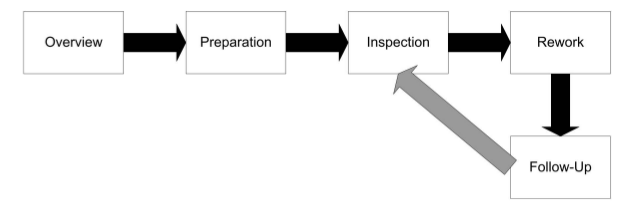
\includegraphics{media/ComparingDefectReductionBenefits}
\caption{The code review process, as described by Fagan \cite{AdvancesInSoftwareInspection} and
reproduced by Wilkerson \cite{wilkerson2012comparing}.}
\label{fig:codeRev:process}
\end{figure}

Furthermore, Fagan \cite{AdvancesInSoftwareInspection} notes that the inspection process should only proceed for 2 hours, since a single developer
can, at best, continue effective code inspection for 2 hours before their defect detection rate
begins to diminish.
He further advocates that there should be a stringent set of roles in the review process, including
\begin{itemize}
	\item the {\em code author}, who prepared the code under review
	\item the {\em reviewer}, who is inspecting the code and finding new errors, and is {\it not} the
		code author
	\item the {\em tester}, who tests the code from a testing standpoint
	\item the {\em inspection moderator}, who facilitates the management of the process, ensures that
		the feedback given to the author is helpful and useful, and above all requires special training
		in their role to maximise their effectiveness
\end{itemize}

Much of the findings in Fagan's paper highlight positive aspects of code reviews.
He notes that software inspections
\begin{itemize}
	\item had long term cost savings over the lifetime of a project, as shown in Figure
		\ref{fig:codeRev:costs}
	\item were more effective than automated testing in finding defects
	\item increased professionalism and developed a culture of cooperation and collaboration amongst
		developers
	\item encouraged more maintainable code that, in the long term, reduced costs even further
\end{itemize}

\begin{figure}
\centering
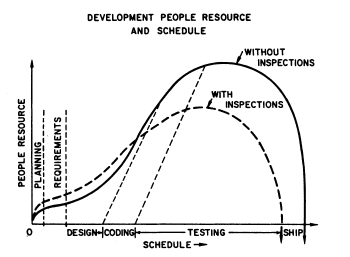
\includegraphics{media/SWInspection_Graph}
\caption{The rate of expenditure, from Fagan's 1986 paper regarding Advances in Software Inspections
	\cite{AdvancesInSoftwareInspection}. Notice that the cost of using software inspections is much
cheaper in the long term than the cost of not using them and simply relying on machine testing.}
\label{fig:codeRev:costs}
\end{figure}

I think Fagan presented code reviews as a revolutionary and must-do technique.
In hindsight, it is perhaps somewhat obvious the code reviews are good --- why not have lots of
people work on, and contribute to improving code?
In the words of Raymond, ``given enough eyeballs, all bugs are shallow" \cite{raymond1999cathedral}.
Although this adage applies to open-source software, a similar mentality can be applied to any
software engineering industry.
Thus, I would say that Fagan presents the obvious --- code reviews are good for software --- and
supports his claims with evidence, as well as formalised procedures to make code reviews an
actionable part of the software development industry.

\section{Analysing Fagan's reviews} \label{sec:litsurvey:strWeak}

Fagan described code reviews in a formal manner --- he outlined a process with strict guidelines and
time limits.
Doolan \cite{doolan1992experience} notes that the process produced a positive benefit upon the
standard and quality of the software his team produced.
We might suggest that Fagan's process of strict processes and formalities was ideal, and had
convincing evidence to suggest that it was well-worth using.\\
\\
But this was in 1986.
The software industry has changed since Fagan's seminal work was published, and we ought to describe
some of the strengths and weaknesses that Fagan's code reviews have shown during this time.
I will raise two points regarding potential gaps in Fagan's advocations.\\
\\
Firstly, the need to have established roles in Fagan's software inspections was something that was
well-motivated at the time.
However, the necessity of an ``inspection moderator" appears to have been lost on the modern
software engineering industry, in my opinion.
Furthermore, having only 2 hour inspection sessions, well-divided segments for the software inspection process
and a process that was reminiscent of a lifecycle approach to designing software suggests that
Fagan's formal software inspection was not particularly appealing to today's lightweight processes
software engineering industry.\\
\\
Fagan prescribed advanced training and coaching for the inspection moderator, but the expense
required to train a person would be counter-intuitive to setting up code reviews.
Perhaps this might be seen to go against the Agile Manifesto's decree of ``people over processes"
\cite{fowler2001agile}, but nevertheless it contributes to a perception that Fagan's code reviews are heavier
processes that are difficult to integrate with other development methodologies (especially those in
the ``Agile" class of development processes).\\
\\
Secondly, Fagan did not discuss reviewer training --- he merely advocated that there needed to be
reviewers and that there should be a guideline of defects that they should look for.
However, reviewers have different levels of experience and competency, and the difference between
developers in terms of effort expended to finish a programming task can sometimes be as much as more
than a factor of 15, according to lectures for this unit.
The competency of the reviewers was not discussed, nor was the issue of how might the guidelines
that a reviewer uses affect their ability to review effectively.\\
\\
I think this is a sound practice to use as software grows larger and evolves in complexity, but
Fagan does not present any empirical evidence (as far as I can tell) that supports his argument.
Nevertheless, my own opinion (from {\em only} reading Fagan's paper) suggests that a guideline is a
good idea, and one that can help guide inexperienced reviewers, as well as focus or remind a more
experienced reviewer about what possible code faults they should be looking for.\\
\\
In criticising Fagan's software inspections, it is also important to acknowledge the gaps in
verification practices that they filled.
It is clear that relying on someone besides the developer to verify the correctness of a software
module clearly addresses some of the shortcomings that some of the verification methods we mentioned
when reviewing the defect detection and prevention techniques.
They do have a somewhat high initiation cost --- you do not need to be an expert in an esoteric field
or uncommon software packages to be a code reviewer, but training an effective review moderator is
not an obvious investment to make.\\
\\
One critical point that Fagan makes is that defects are found earlier, using software inspections.
He adds that some studies, such as Crossman \cite{crossman1977some} improve developer cohesion as a
team, and the developer culture overall.
Furthermore, he notes how the lessons learnt from code reviews, like any kind of review (such as a
P.I.R. or the ideas of first-order and second-order change, as discussed in this course), produce
results and {\em feedback}, which can constructively be used to improve future development and code.
This is an important part of defect prevention, which speaks to the wider ability of code reviews to
effect cultural changes and improve procedures.\\
\\
Finally, we ought to speak to our last point regarding considering a system in its overarching
design and architecture.
Fagan's reviews suggested that humans read through code for 2 hours, and provide feedback on how
effective the change was.
However, Fagan's paper advocates for stages such as {\em preparing} for the inspection, as well as
a {\em follow-up} to check on how the changes have been implemented.
In my opinion, this suggests that such preparation would help the reviewers and verifiers to get a
larger, high-level overview of the software architecture and how a change to the code improves the
software system as a whole.\\
\\
It is unclear whether such preparation could help when software has spiralled into such a large
entity.
Code-bases can be hundreds of thousands of lines of code --- this is a huge amount for an inspection
team to prepare for.
Placing the burden on a small number of reviewers to consider changes that could affect large sections
of the code base is a difficult issue to deal with.
As a result, I feel like this complexity questions the relevance of code reviews with regards to verifying
high-level architectural designs in today's software industry.

\section{State of the art} \label{sec:litsurvey:current}

Let us fast-forward from analysing Fagan's 1986 reviews --- it is now almost 30 years since Fagan's
seminal work.
What does the literature say about code reviews now?\\
\\
For one thing, much of the literature no longer ascribes to Fagan's heavier software models.
We note that in a number of studies since Fagan's paper, the concept of a code inspection or review
is ill-defined \cite{siy2001does,cohen2006best,wilkerson2012comparing,grbac2012quantifying}.
The formal software processes for software inspections that Fagan discussed are no longer ascribed
to --- in their place is the concept that a code review is to have someone read code and critically
evaluate it, giving constructive feedback on how the code could be reviewed \footnote{This is an
informal definition that I have constructed, mainly from my own reading of literature.}.\\
\\
We have noticed that the software inspection process is less concretely defined than previously ---
but is this as big a problem as we might expect?
Cohen et. al \cite{cohen2006best} found in their own case study that a tool-assisted software
inspection that was not as rigourously defined as Fagan's could be implemented at a lower cost, and
be just as effective.
So what other major discoveries have we made about code reviews?\\
\\
A major work that I uncovered during my research was performed by Wilkerson et. al
\cite{wilkerson2012comparing}, who compared Test-Driven Development (TDD) to code reviews.
They had three hypotheses regarding how effective code reviews were, compared to test-driven
development.
\begin{enumerate}
	\item  Code reviews were more effective at finding defects than TDD
	\item Code reviews required more effort to implement than TDD
	\item Code reviews, when used together with TDD, are more effective at finding defects than either alone
\end{enumerate}

The authors found that the first two hypotheses both held, but they had to reject the third one.
Interestingly, the authors found an unexplained relationship between code reviews and TDD in terms
of cost that was significant, but unexplained, and they had no proper experimental frameworks to
deal with this, other than to observe that it had occurred.
We ought to note that their findings suggested that code reviews were more effective at
finding defects --- a major point by way ways of code reviews, and confirming their effectiveness.
However, this experiment was done within a student body, and the researchers acknowledged that this
threatened the validity of their results.\\
\\
Our other observation can be made that since this was a short project, it would have been difficult
to see the benefits cost-wise of a code review.
In my opinion, it is clear that it would be difficult to show that software
inspections had a cost-saving element using such short-term experiments.
It would be the longer-term studies that discussed the maintainability of the code, as well as the
defect prevention properties that code reviews had, which would demonstrate their worth in terms of
cost and expenditure.\\
\\
Indeed, such results are discussed by Grbac et. al \cite{grbac2012quantifying}, where they attempt
to quantify the benefits behind inspecting earlier, as opposed to later.
They note that there were drastic improvements in the quality of code that is produced for a project.
The authors did not find that the cost-benefit of introducing code reviews was statistically
significant, but this was done on a single iteration of the development cycle.
The developers were confident that a longer-term study would reveal the lowered maintenance costs of
code reviews.\\
\\
Similar results, with regards to improving the maintainability of code, are shown by Siy and Votta
\cite{siy2001does}.
They ask whether the ``modern" code review, with a loose definition and lack of process, can offer
as much value as before.
In particular, the motivating factor was the change in the software engineering industry --- all the
different types of verification techniques and whether code reviews were still {\it relevant} in
such an environment.\\
\\
Siy and Votta found that the long term maintainability of the code they were studying was greatly
improved by using code reviews.
They acknowledged that code reviews were finding approximately 60$\%$ of the same bugs as machine testing, but
that the remaining bugs that they found using code review alone were detected early, as faults in
the source code.
These faults were prevented from becoming program errors or system failures, and this is important
in determining the long-term power that software inspections possess.\\
\\
I think that here, it is worth noting that we have revealed the implicit power of defect prevention.
Much of what I have written revolves around finding defects --- the number of defects uncovered, or
that 2 hours of inspection is the optimal time to maximise the number of defects found.
But software inspections true power, in my opinion, relates back to fixing a problem early, when it
is still a fault in the code, and when it is yet to impact the system as an error or failure.
It is the code review that finds these defects early, combining static analysis with critical
thinking and human insight to determine whether a fault exists.\\
\\
Many of these outcomes might already be achievable with automated static analysis.
Finding bad code smells and practices, or spell-checking documentation, are defects that a good
static analysis package can do.
Circular dependencies might be detectable using good static analysis software.
However, I do not believe that maintainability issues and subtle defects are so easily found with
static analysis.
These defects, which {\it may} arise in the future as a result of small changes that we make now,
are the kinds of defects that a software inspection can find.
This is my opinion, supported by both Siy and Votta \cite{siy2001does} and Grbac et. al
\cite{grbac2012quantifying} --- that the number of defects in software, both now and in the future,
is lower as a result of code inspections.\\
\\
Aurum et. al \cite{aurum2002state} perform a somewhat dated, but far-reaching survey in their own
work regarding the state of the art of code reviews.
They examined a number of different code review techniques (older techniques which I did not find
much mention of in the recent literature I surveyed), such as
\begin{itemize}
	\item phased inspections, which divide an inspection into phases and examine code in a phase
		against a certain criteria
	\item $n$-fold inspections, which use $n$ parallel teams of inspectors to find as many as bugs as
		possible
\end{itemize}

Aurum's work also examines the different techniques for improving code reviews as
well.
Of particular interest were the different kinds of reading techniques, which assist in improving inspections --- the
authors noted that there were two different kinds of reading techniques, a {\em structured
reading technique}, which presented a clear framework to carry out the inspection within, and an
{\em unstructured reading technique}, which relied on the reviewer's intuition.\\
\\
Examples of reading techniques included
\begin{itemize}
	\item ad-hoc reading --- or no guidance, which appears to be the main trend today
	\item checklists, a reading technique which Fagan \cite{AdvancesInSoftwareInspection} also
		advocated, was a list of defects to look for and try to detect
	\item defect-based reading --- where a set of scenarios are constructed for the purposes of
		determining if a defect exists, and a reviewer answers questions about the scenarios in
		order to ascertain the existence of a defect
\end{itemize}

I did not look further into advances in reading techniques, unfortunately, since Aurum's work was
one that I happened upon rather late into my investigations.
Given more time, I would like to explore and follow up on the avenues of research he found.
I would again present my own opinion with regards to structured, compared to unstructured reading
techniques, and claim that the unstructured techniques would be more useful or valuable.
I would suspect that unstructured techniques would not limit the creativity and inquisitiveness in the
way a structured technique, and its frameworks and forced conceptions might.\\
\\
However, it might also be the case that depending upon which kind of software we are developing, the
reading technique we want to use ought to differ.
This is a reasonable viewpoint that Aurum takes, and acknowledges the relative strengths and
weaknesses of each technique.
It brings us to some of the gaps in knowledge that still exist in code reviews.

\section{Open questions}

Here, I hope to highlight some of the open questions that I feel have been elicited through my
survey, and thus motivate a series of experiments that might contribute to filling this gap in
knowledge

\begin{itemize}
	\item It is almost 30 years since Fagan's seminal review, and 10 since Aurum's review. Electronic
		support for code reviews was still in its fledgling stages, and it was stated that the support
		had little to no effect upon inspection effectiveness. How has that changed since then? Have
		reviews become better or worse because of code review tools such as the one provided on GitHub
		becoming readily available?
		For both the commercial software industry, and for the new and relatively unstudied field of open source software?
	\item Much of the recent work done has begun to look at how code reviews are affected by other
		defect detection and prevention techniques.
		One technique that code reviews does not appear to have been compared against is defensive
		programming --- how do the two affect each other?
		Will a defensive programming-styled program be more difficult or easier to review?
	\item We note that Wilkerson et. al \cite{wilkerson2012comparing} observed interplays of cost
		between TDD and code reviews. Why? It was a question that Wilkerson et. al were not prepared to analyse
		and their experimental framework was not able to effectively capture or deduce the reasons why.
		It would be worthwhile to thus revisit this interplay and try and determine how the two are
		related.
	\item How does the problem domain affect the quality of a review? For example, would the review
		and defects to be detected in a web-based application differ from a safety critical system? Most
		certainly! But how, and why? Are there a set of best practices that can be elicited that we
		ought to follow, depending upon the project?
	\item What is the overlap between automated static analysis and code reviews? I did not actually
		look into this deeply, but I think it is an interesting and useful question. It is easily
		motivated by the ability to optimise code reviews to not have to find defects that automated
		analyses can find already, and instead focus on subtler issues of design and maintenance that an
		automated analysis might miss.
\end{itemize}
